\hypertarget{haskell}{%
\section{Haskell - Declaring Types and Classes}\label{haskell}}

\hypertarget{type-declarations}{%
\subsection{Type Declarations}\label{type-declarations}}

In Haskell, a new name for an \textbf{existing} type can be defined
using a type declaration. (not new type)

\begin{lstlisting}[language=Haskell]
type String = [Char]
--or
type Pos = (Int,Int)
\end{lstlisting}

Like function definitions, type declarations can also have parameters.
For example, given

\begin{lstlisting}[language=Haskell]
type Pair a = (a,a)
\end{lstlisting}

Type declarations can be nested, but not recursive.

\begin{lstlisting}[language=Haskell]
--Allowed
type Pos = (Int,Int)
type Trans = Pos -> Pos

--Not allowed
type Tree = (Int,[Tree])
\end{lstlisting}

\hypertarget{data-declarations}{%
\subsection{Data Declarations}\label{data-declarations}}

A completely \textbf{new} type can be defined by specifying its values
using a data declaration.

\begin{lstlisting}[language=Haskell]
data Bool = False | True
\end{lstlisting}

\begin{itemize}
\tightlist
\item
  The two values False and True are called the constructors for the type
  Bool.
\item
  Type and constructor names must always begin with an upper-case
  letter.
\item
  Data declarations are similar to context free grammars. The former
  specifies the values of a type, the latter the sentences of a
  language.
\end{itemize}

\hypertarget{constructor}{%
\subsubsection{Constructor}\label{constructor}}

The constructors in a data declaration can also have parameters. For
example, given

\begin{lstlisting}[language=Haskell]
data Shape  = Circle Float
            | Rect Float Float
\end{lstlisting}

we can define

\begin{lstlisting}[language=Haskell]
square :: Float -> Shape
square n = Rect n n
area :: Shape -> Float
area (Circle r) = pi * r^2
area (Rect x y) = x * y
\end{lstlisting}

Not surprisingly, data declarations themselves can also have parameters.
For example, given

\begin{lstlisting}[language=Haskell]
data Maybe a = Nothing | Just a
\end{lstlisting}

we can define

\begin{lstlisting}[language=Haskell]
safediv :: Int -> Int -> Maybe Int
safediv _ 0 = Nothing
safediv m n = Just (m `div` n)
safehead :: [a] -> Maybe a
safehead [] = Nothing
safehead xs = Just (head xs)
\end{lstlisting}

\hypertarget{recursive-types}{%
\subsection{Recursive Types}\label{recursive-types}}

In Haskell, new types can be declared in terms of themselves. That is,
types can be recursive.

\begin{lstlisting}[language=Haskell]
data Nat = Zero | Succ Nat
--Nat is either zero or a successor of Nat
\end{lstlisting}

e.g.~Succ (Succ (Succ Zero)) = 3.

\hypertarget{binary-trees}{%
\subsection{Binary Trees}\label{binary-trees}}

A binary tree is a two-way branching structure. Using recursion, a
suitable new type to represent such binary trees can be declared by:

\begin{lstlisting}[language=Haskell]
data Tree a = Leaf a
            | Node (Tree a) a (Tree a)
\end{lstlisting}

\begin{figure}[H]
\centering
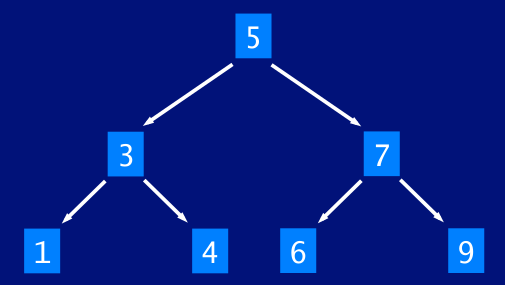
\includegraphics[width=0.5\textwidth]{figures/binaryTreeExample.png}
\caption{Tree Example}
\end{figure}

This tree could be represented with

\begin{lstlisting}[language=Haskell]
t :: Tree Int
t = Node (Node (Leaf 1) 3 (Leaf 4)) 5
(Node (Leaf 6) 7 (Leaf 9))
22
\end{lstlisting}

\clearpage